\documentclass[brazil,a4paper,12pt]{article}

\usepackage{fullpage}
\usepackage{fancyvrb}
\usepackage[brazil]{babel}
\usepackage[utf8]{inputenc}
\usepackage{graphicx}
\usepackage{booktabs}
\usepackage{subfigure}

\begin{document}

\begin{center}
\LARGE
\textbf{Mineração de Dados}\\
\textbf{TP3: Song Clustering}\\
\end{center}
\begin{center}
\textbf{Aluno: Flavio Vinicius Diniz de Figueiredo}
\end{center}

\section{Descrição}

O objetivo do TP foi de realizar as seguintes o agrupamento de musicas
similares de uma base coletada do LastFM~\footnote{\texttt{http://www.last.fm}}.
De forma resumida foi requisitado do aluno:

\begin{description}

\item [Proposta de Técnica] O aluno deveria propor uma técnica de agrupamento de
dados para gerar os grupos de músicas similares. O TP deixou claro que deveria-se
identificar grupos distintos de música, ou seja, cada música pertence a um grupo
apenas. Ao entender do aluno, esta etapa inclui não apenas a implementação de um
algoritmo de agrupamento, será necessário: (1) fazer o pre-processamento de dados;
(2) escolha da melhor forma de representar os dados; (3) determinação do número de
grupos a serem extraídos; e por fim, (4) escolha do algoritmo de agrupamento.

\item [Proposta de Avaliação] Determinar ser uma técnica de agrupamento é eficaz
para agrupamento é um problema ainda em aberto. Existem diversas heurísticas que
visam sumarizar características intuitivamente relevantes do agrupamento, porém
o uso adequado destas depende da base de dados e técnica utilizada. Sabendo disto,
foi requisitado do aluno a proposta de uma estratégia de avaliação da qualidade dos
grupos encontrados.

\end{description}

\noindent Como foi requisitado o código utilizado no TP, no fim de cada seção 
indicamos quais arquivos contém os scripts utilizados na implementação e avaliação 
da técnica.

\section{Limpeza de Dados}

O conjunto de dados originais era composto de 191538 músicas coletadas do LastFM.
Cada música é representada pelo conjunto de tags mais utilizadas por usuários para
descrever a mesma no sistema. Iniciamos a análise dos dados fazendo os seguintes
pré-processamentos:

Para limpeza de dados foram realizadas as seguintes etapas~\footnote{Uma etapa extra
de desconsiderar tags muito raras ou muito frequentes, considerando a quantidade de
músicas anotadas, também foi realizada. Porém, esta trouxe pouca diferença nos resultados
do agrupamento. Para os resultados do relatório não realizamos tal filtro.}:

\begin{enumerate}
\item Inicialmente identificamos as tags que anotaram cada música. Após
isto, colocamos todas estas tags em {\it lowercase}. Para identificar
as tags em cada músicas, consideramos apenas as tags compostas por
caracteres alfanuméricos ($[a-zA-z0-9]+$).

\item Após isto, filtramos as {\it stopwords} da língua
inglesa. Como tais palavras são muito frequentes e trazem pouca
informação, é geralmente recomendado o filtro destas.

\item As palavras restantes foram removidas de afixos. Isto é, convertemos
as palavras para a sua sua raiz morfológica mais simples. Para isto, 
utilizamos o algoritmo de Porter Stemmer~\footnote{
\texttt{http://tartarus.org/martin/PorterStemmer/}}~\cite{baeza2010modern}.

\item Se após as etapas anteriores, todas as tags da músicas tivessem sido
filtradas, nós desconsideramos a música da nossa base.

\end{enumerate}

\begin{figure}
\centering
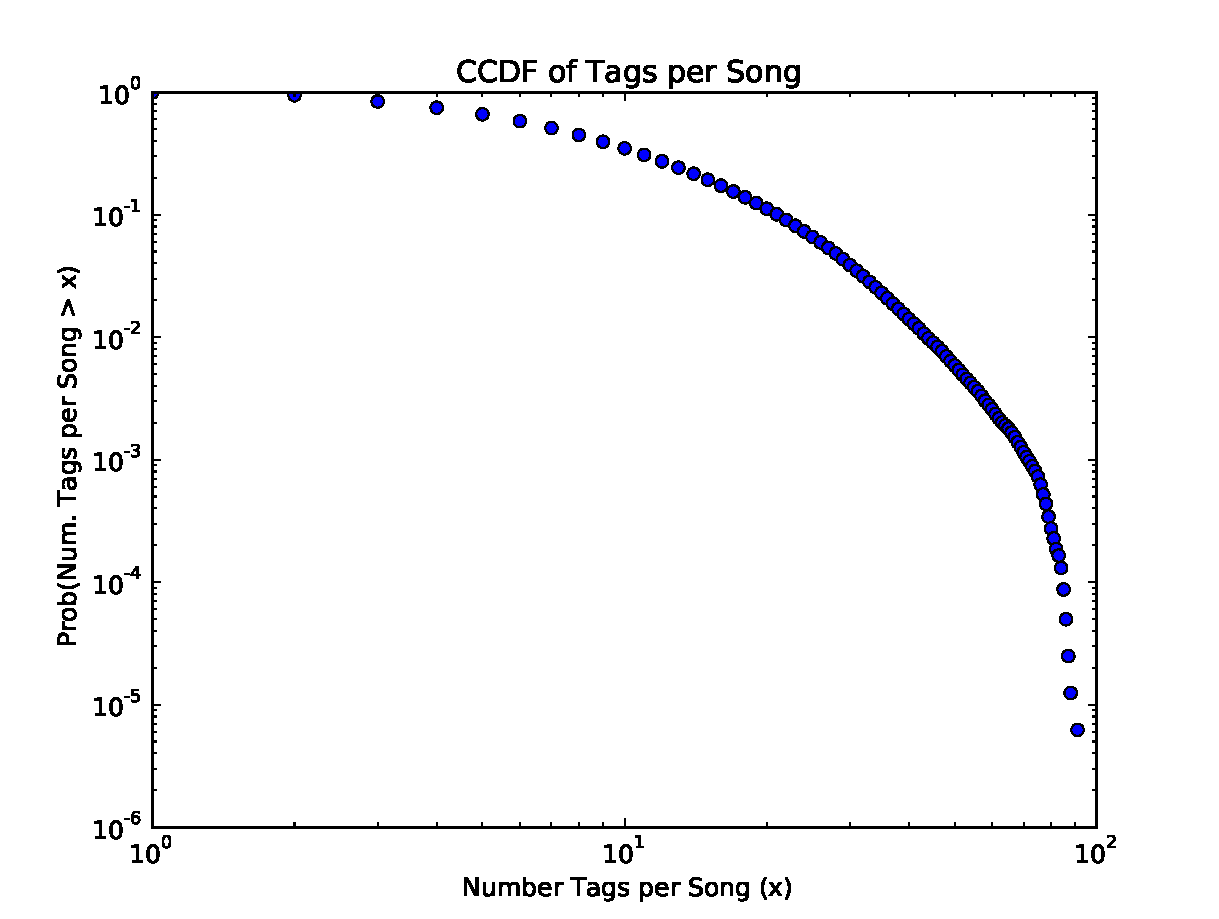
\includegraphics[scale=0.6]{tps.pdf}
\caption{CCDF do número de tags em por música}
\label{fig:tps}
\end{figure}

\begin{figure}
\centering
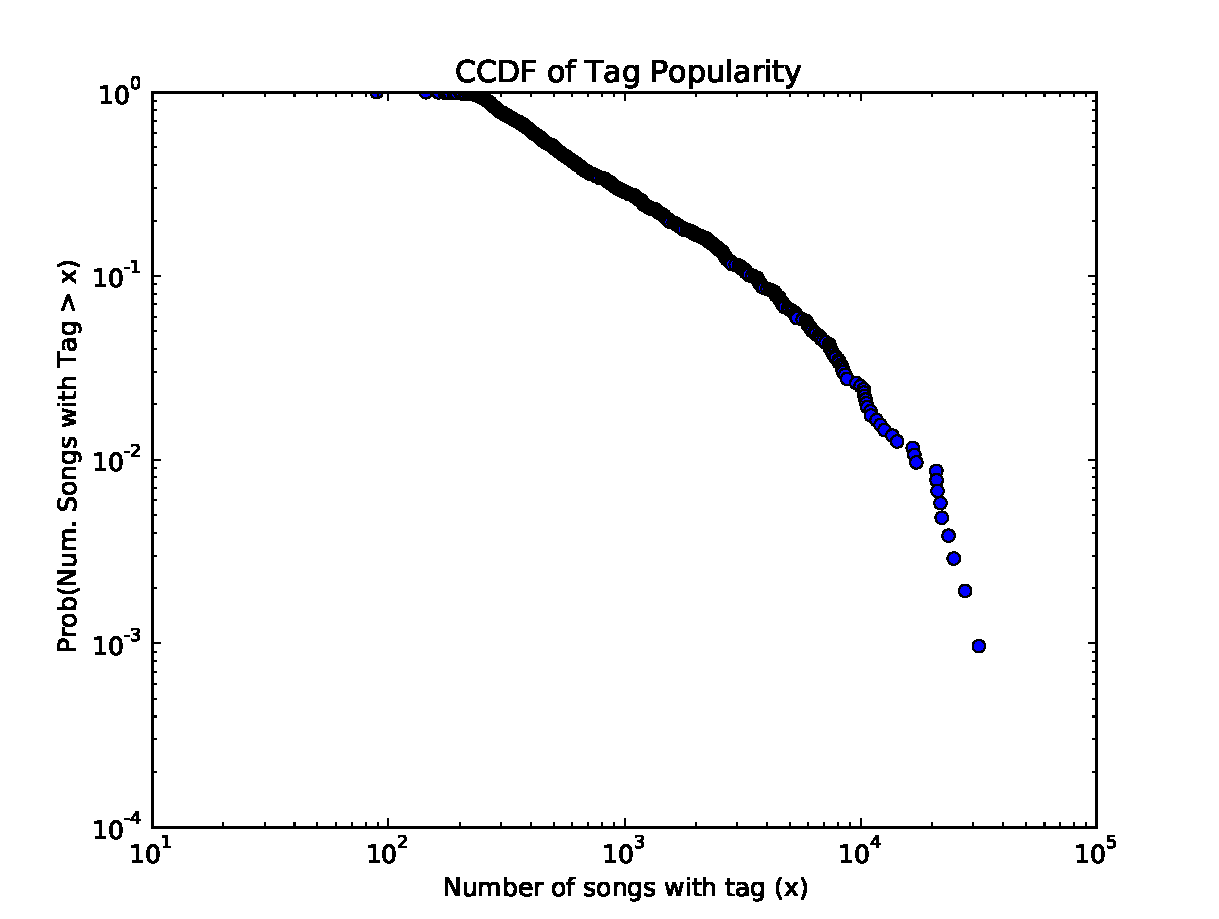
\includegraphics[scale=0.6]{tpop.pdf}
\caption{CCDF da popularidade das tags}
\label{fig:poptags}
\end{figure}

Tais técnicas são padrões no tratamento de dados textuais 
tanto para mineração de dados como para recuperação de informação.
Para mais detalhes, 
ver o Capítulo 6.6 do livro Modern Information Retrieval~\cite{baeza2010modern}.

Após o pré-processamento, restaram 160734 músicas e 1036 tags distintas na base.
A Figura~\ref{fig:tps} mostra o complemento da distribuição cumulativa de
probabilidade (CCDF) do números de tags por música. Pela figura, 
podemos ver que nenhuma música contém mais do que 100 tags. A maioria delas
(90\%) contem ao máximo 3 tags. A Figura~\ref{fig:poptags} mostra o complemento 
da distribuição cumulativa de probabilidade (CCDF) da quantidade de músicas anotadas 
por cada tag.  Na figura, podemos ver que a tag mais popular chega a anotar mais que 
10000 músicas, enquanto metade delas anota mais do que 173 músicas. Isto é esperado,
dada a baixa quantidade de tags em relação às músicas.

Até o momento podemos concluir que: (1) tags são frequentemente reutilizadas
entre músicas; (2) músicas no gera contém poucas tags, em sua maioria apenas 2 tags. 
Acreditamos que estes dois fatos são devido a forma de coleta dos dados, na documentação
foi mencionado que tais tags eram apenas as mais frequentes por músicas e não todo o conjunto
de tags no sistema.

\subsection{Código}
\begin{verbatim}
src/dm/tp3/lastfm_io.py
src/dm/tp3/scripts/convert_data.py
src/dm/tp3/scripts/plot_num_tags_per_song.py
src/dm/tp3/scripts/plot_tag_dist.py
\end{verbatim}

\section{Número de Grupos e Representação dos Dados}

Para realização do TP decidimos fazer uso do algoritmo 
\emph{Mini Batch K-Means}~\cite{sculley2010web}. O motivo da escolha deste
algoritmo é que o mesmo já foi demonstrado como adequado para grandes base
de dados esparsas no passado. Em especial, o algoritmo foi desenvolvido
justamente com o foco de clusterização de base de dados Web como a 
base do TP. A implementação utilizada foi a da biblioteca 
{\bf scikits.learn}~\footnote{\texttt{http://scikit-learn.sourceforge.net/}}.

\subsection{Representação dos Dados}

Como cada música é composta de um conjunto de palavras, decidimos representar
a base usando o modelos vetorial~\cite{baeza2010modern,meira}. Nesta representação,
cada música será composta de um vetor esparso onde os elementos do vetor representam
cada termo. Isto é:

$$ \mathbf{s} = <{w_1, w_2, w_3, \cdots}>, $$

onde $w_i$ é o peso do termo na música. Para definir este peso escolhemos
entre duas alternativas:

\begin{description}

\item [Pesos binários] Nesta abordagem, o peso de cada termo é apenas 1 ou 0
caso o termo apareça ou não na música.

\item [TDIDF] Nesta abordagem, o peso da música é determinada pelo seu valor
$TF-IDF$~\cite{baeza2010modern}. Como tags são únicas nas músicas, o fator
IDF domina este peso.

\end{description}


\begin{figure*}[t!]
 \centering
 \mbox{\subfigure[Pesos Binários]{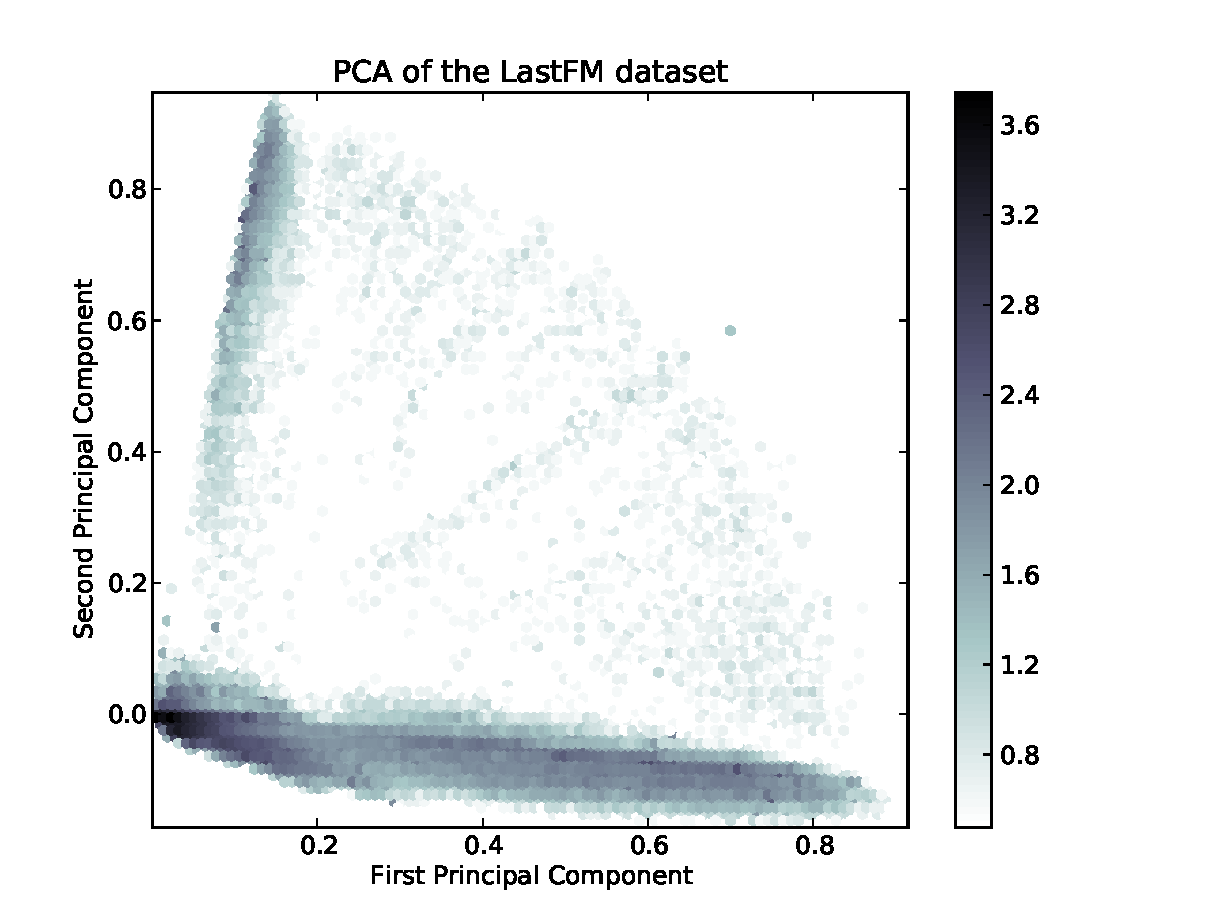
\includegraphics[width=0.48\linewidth]{pca_noidf_nofilt.pdf}}}
 \mbox{\subfigure[TFIDF]{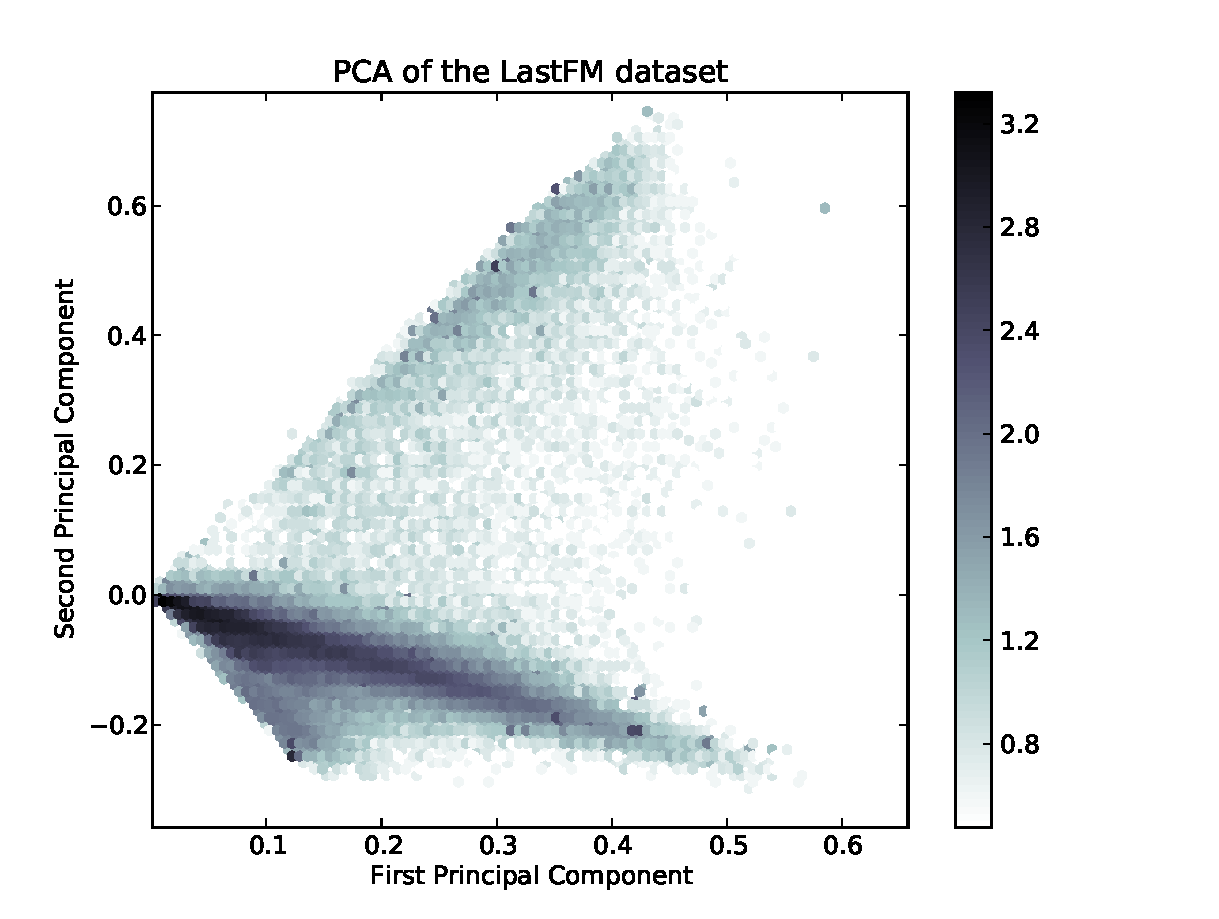
\includegraphics[width=0.48\linewidth]{pca_idf_nofilt.pdf}}}
 \caption{Scatter plot dos dois principais componentes dos dados}
 \label{fig:pca}
\end{figure*}

Para escolher entre as duas estratégias, fizemos uso de PCA para plotar os dois
componentes principais dos dados. Esta é um técnica recomendada para visualização
de dados em mais de duas dimensões~\cite{alpaydin2010introduction}. 

A Figura~\ref{fig:pca}(a) demonstra os dois principais sem o uso de TFIDF, em 
contrapartida a Figura~\ref{fig:pca}(b) demonstra os mesmos componentes com o
uso de TFIDF. Cada figura é um scatter plot dos dois principais componentes dos dados. 
Cada eixo das figuras representa um componente. Para facilitar a visualização, 
agrupamos~\footnote{Não confundir com o agrupamento de clustering, problema do TP} 
as músicas muito próximo uma das outras no plot, o log da densidade 
determinada grupo é determinado pelas cores. Pelas figura, é possível visualizar
uma melhor separação dos dados com o peso binário, quando o mesmo é utilizado
os dados ficam mais embaralhados em dois ou três grande grupos. Este resultado
é condizente com a literatura que indicam que o uso de IDF impacta de forma 
negativa a eficácia de tarefas de agrupamento~\cite{ramage2009ctw,haveliwala2002ess}.

Um outro resultado mais fraco, porém interessante, de se ver na Figura~\ref{fig:pca}(a),
é o possível formato dos grupos em duas dimensões. Aparenta que em duas dimensões os
grupos são elipses, existindo dois grandes grupos de vídeos e outros menores.

\subsection{Número de grupos}

\begin{figure}
\centering
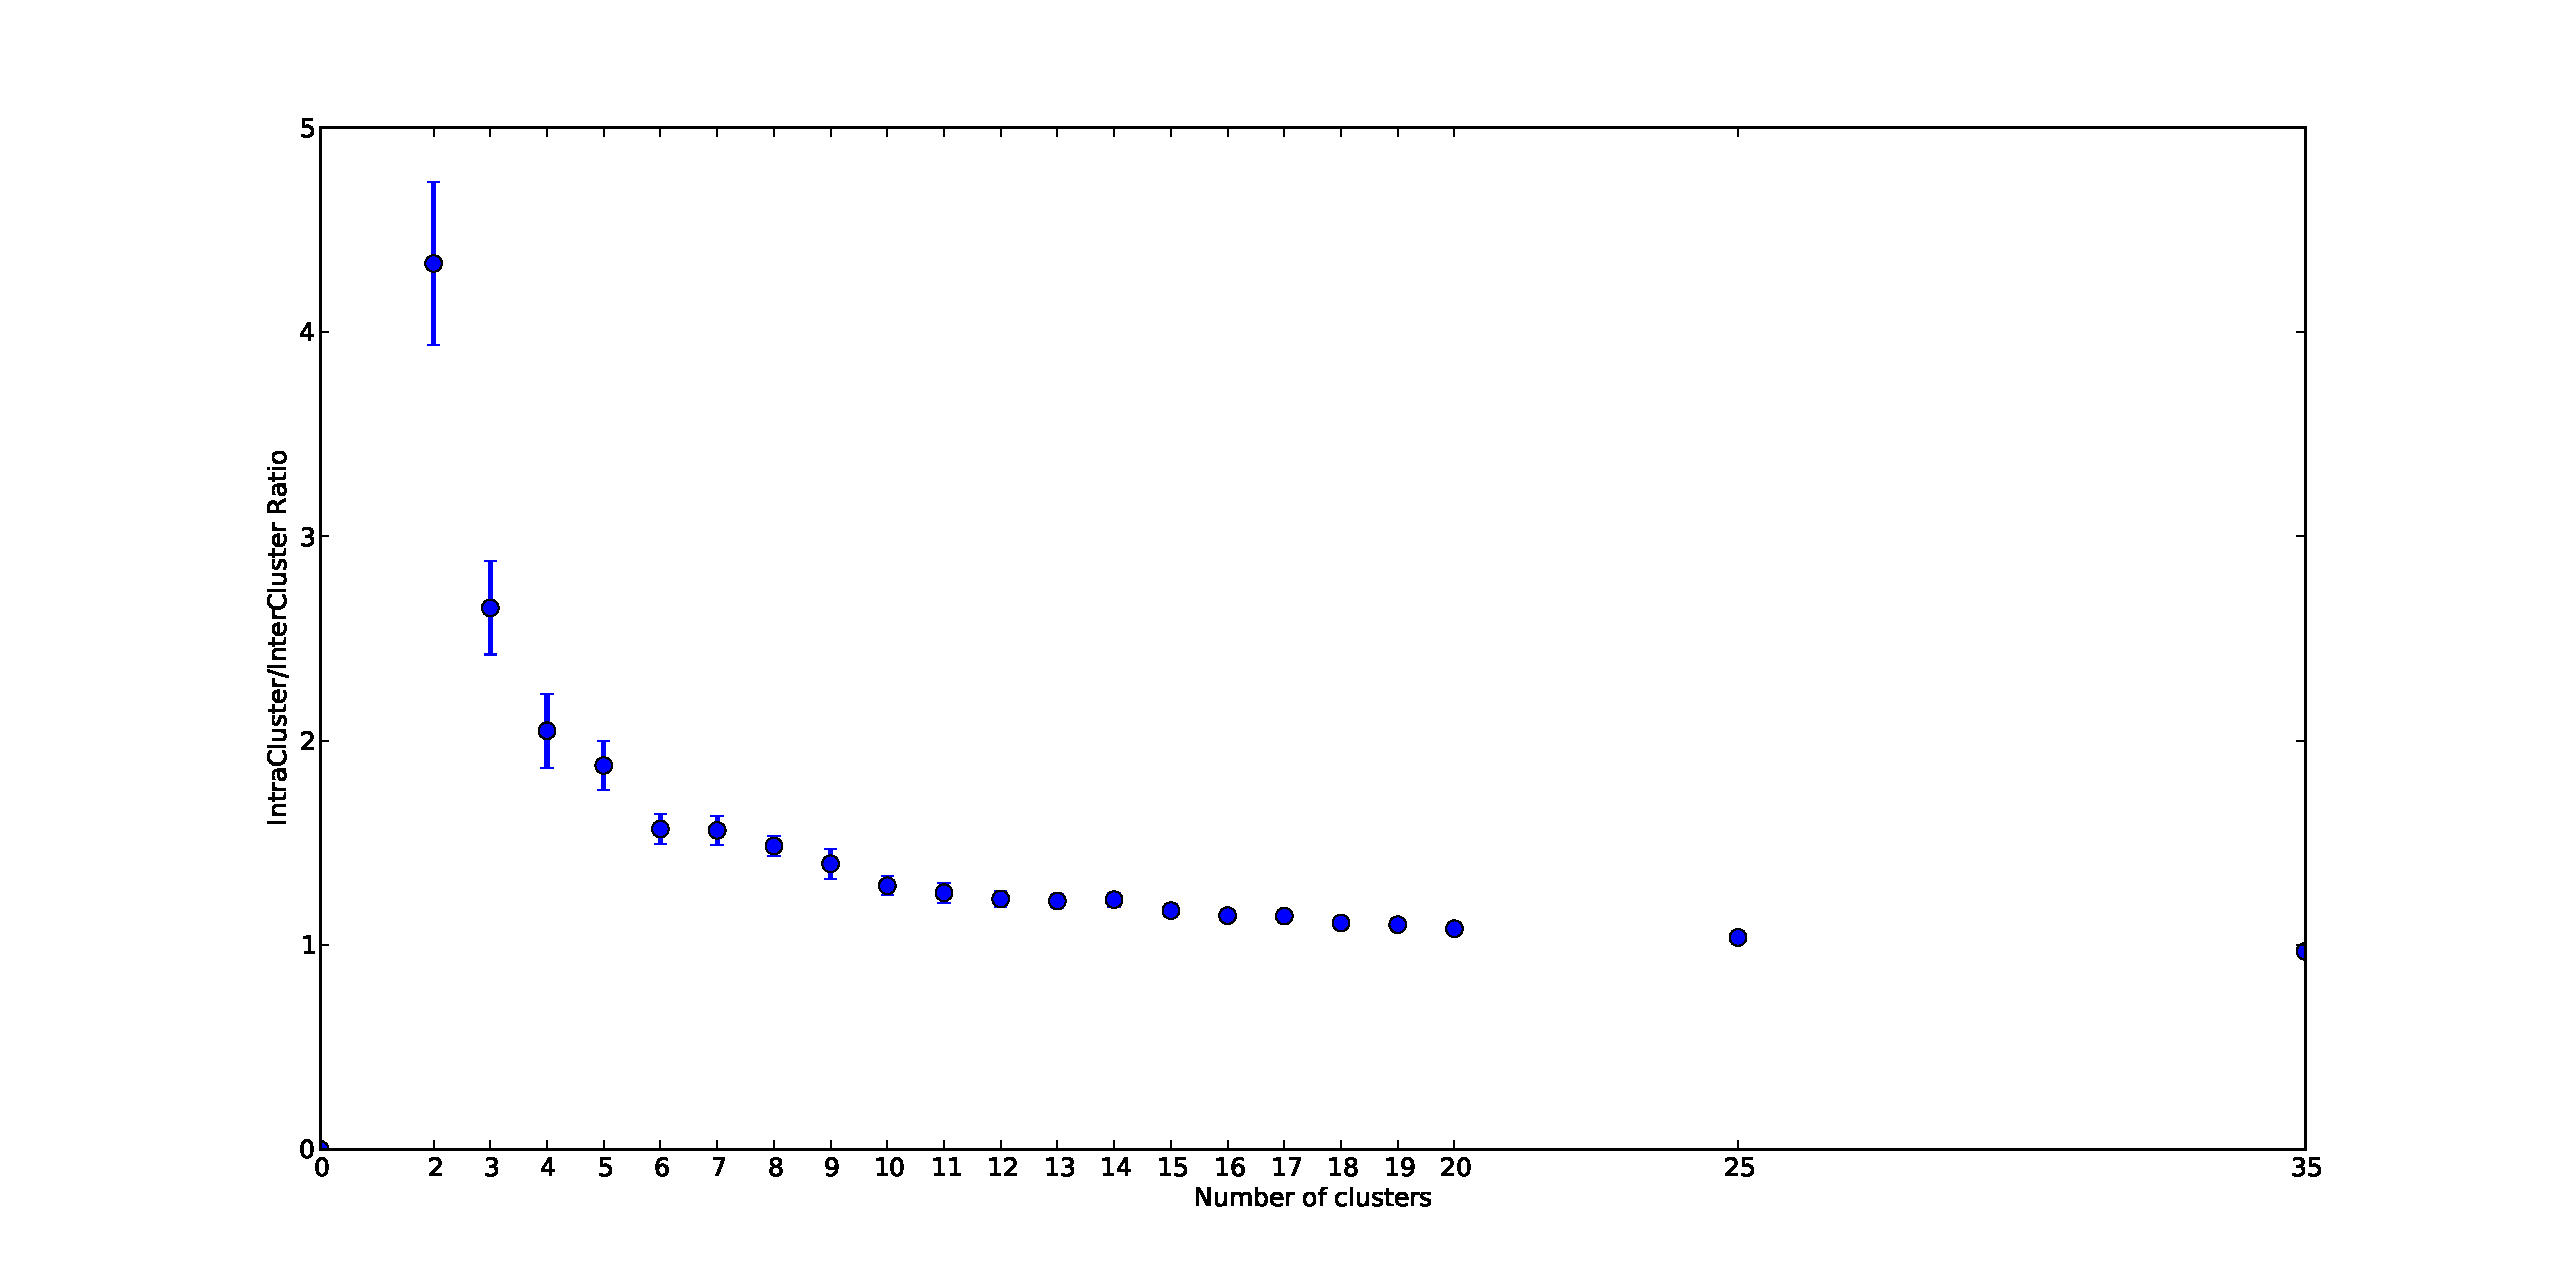
\includegraphics[scale=0.4]{betacv.pdf}
\caption{Razão das distâncias intra e inter grupos}
\label{fig:betacv}
\end{figure}

Um dos problemas do uso de variações do \emph{K-means} é a escolha do número de 
grupos. Para resolver este, executamos 10 vezes o algoritmo para diferentes valores 
número de grupos (k). Após a execução, analisamos a razão média entre: (1) a distância de cada 
documento para seu grupos; com (2) a distância entre os centros do grupos. A média deste valor
para as 10 execuções com o intervalo de confiança, usando 90\% de confiança, 
está representada na Figura~\ref{fig:betacv}. Esta técnica está descrita com mais detalhes no livro
Perfomance by Design~\cite{menasce2004performance}.

Pela figura, podemos ver que após $9$  grupos a razão computada estabiliza. Como a ideia do
agrupamento é maximizar a distância  inter grupos (1) e minimizar as distâncias internas 
dos grupos (2), pode se dizer que qualquer valor após $9$ tem a mesma qualidade. 
Por isto, escolhemos como $9$ o número de grupos. Foi surpreendente constar que este
número de grupos é justamente o número de classes encontradas para uma outra base
do LastFM em um trabalho passado~\cite{figueiredo2009evidence}. Um indicativo de que este
pode ser considerado como correto.

\subsection{Código}

\begin{verbatim}
src/dm/tp3/scripts/betacv.py
src/dm/tp3/scripts/k_means.py
src/dm/tp3/scripts/plotpca.py
\end{verbatim}

\section{Avaliação dos Agrupamentos}

A última etapa do TP era referente a avaliação da qualidade dos grupos gerados. Inicialmente
nós executamos 10 vezes o algoritmo do \emph{Mini Batch K-Means} para gerar 10 agrupamentos
de 9 grupos distintos. Para cada música, escolhemos como seu grupo como sendo o grupo que mais
ocorreu nas 10 execuções do algoritmo. Além disto, descartamos os objetos cujo o grupo mais frequente
das 10 execuções ocorreu duas ou menos vezes. Este procedimento foi feito para reduzir o efeito da aleatoriedade do algoritmo.

O procedimento acima foi realizado usando duas bases. Inicialmente executamos este na base filtrada e
após isto executamos o mesmo utilizando como base os 10 componentes principais da base. Isto foi feito
para reduzir os problemas devidos ao mal da dimensionalidade~\cite{meira}. A Tabela~\ref{tab:clus} e 
~\ref{tab:cluspca} mostra a quantidade de músicas em cada grupo para a execução sem o uso de PCA (NONPCA) e e com o uso de PCA respectivamente (PCA). Embora os grupos compartilhem do mesmo
$ClusterID$ nas duas execuções, não podemos afirmar que semanticamente eles são o mesmo grupo.
No total 58589 e 89868 objetos foram desconsiderados para a análise NONPCA e PCA respectivamente.

\begin{table}
\centering
\small
\begin{tabular}{cc}
\toprule
ClustID & Número de Músicas  \\
\midrule
6	&	29396 \\
3	&	18794 \\
0	&	13679 \\
5	&	11962 \\
1	&	9443 \\
8	&	6004 \\
7	&	5916 \\
4	&	5875 \\
2	&	1076 \\
\bottomrule
\end{tabular}
\caption{Números de músicas por cluster (NONPCA)}
\label{tab:clus}
\end{table}

\begin{table}
\centering
\small
\begin{tabular}{cc}
\toprule
ClustID & Número de Músicas  \\
\midrule
0	&	24909 \\
5	&	19784 \\
8	&	8123 \\
1	&	7357 \\
4	&	3883 \\
6	&	3351 \\
3	&	1877 \\
2	&	1450 \\
7	&	132 \\
\bottomrule
\end{tabular}
\caption{Números de músicas por cluster (PCA)}
\label{tab:cluspca}
\end{table}

\subsection{Entropia de Grupos}

Para mensurar a qualidade de agrupamentos, decidimos computar o a coesão do grupo através da
entropia dos termos que compõem aquele grupo. A entropia mensura a quantidade de bits necessários
para codificar a informação contida em uma distribuição de probabilidade, sua fórmula é:

$$ H(X) = -1 \times \sum_{x \in X} p(x) \times log2(p(x)),$$

\noindent consideramos como variável aleatória ($X$) a probabilidade to termo ocorrer dado
que o grupo ocorreu, isto é:

$$ p(t | C = c) =\frac{p(t, c)}{p(c)}, $$

onde $p(t, c)$ é a probabilidade conjunta do grupo e tag; e, $p(c)$ é a probabilidade do 
grupo. Estes dois fatores podem ser estimados usando estimadores de {\it maximum likelihood}. Em
outras palavras, são deduzidos a partir da frequência dos termos e dos grupos na base de dados. 
Notamos que no nosso caso, menor entropia é melhor, indicando que o grupo é mais coeso e necessita
de menos bits para codificar.


\begin{table}
\centering
\small
\begin{tabular}{cc|l|l}
\toprule
ClustID & H & Tags Mais Frequentes & Tags Mais Prováveis \\
\midrule
\textbf{6}	& \textbf{49.54} & \textbf{electron, pop, electronica, danc, vocalist} & t\textbf{ranc, psybient, psi, goa, psychil} \\
3	& 50.15 &          rock
         classic
         pop
         hard
         progress &          protopunk
         chameleon
         sleaz
         invas
         glam  \\
\textbf{0}	& \textbf{41.41} & \textbf{hop, hip, rap, soul, underground} & \textbf{strictli, wu, tang, hip, gangsta}  \\
\textbf{5}	& \textbf{41.86} &          \textbf{metal
         rock
         black
         heavi
         melod}
 &       \textbf{vike
         pagan
         speed
         front
         symphon}
 \\
1	& 52.46 & song, love, music, favorit, rock & contest, eurovis, motown, prais, lined  \\
8	& 51.99 &          indi
         rock
         altern
         pop
         favorit &          britpop
         brit
         manchest
         creek
         indi  \\
7	& 52.45 &          indi
         rock
         pop
         altern
         love & nix
         chamber
         indiepop
         6
         creek  \\
\textbf{4}	& \textbf{42.73} & \textbf{rock
         punk
         altern
         pop
         favorit} & \textbf{skate
         punkrock
         deutschpunk
         anarcho
         oi}  \\
2	& 60.27 & altern, vocalist, femal, rock, indi & ethinic, indian, chick, arab, world  \\
\bottomrule
\end{tabular}
\caption{Números de músicas por cluster (NONPCA)}
\label{tab:hnonpca}
\end{table}

\begin{table}
\centering
\small
\begin{tabular}{cc|ll}
\toprule
ClustID & H & Tags Mais Frequentes & Tags Mais Prováveis \\
\midrule
0	&	63.06 &          rock
         altern
         indi
         pop
         song & brit
         britpop
         colleg
         ben
         indi  \\
\textbf{5}	&	\textbf{45.39} & \textbf{electron
         electronica
         ambient
         electro
         danc} & \textbf{psybient
         psychil
         emp805
         idm
         minim}  \\
8	&	64.76 & jazz
         indi
         instrument
         funk
         acid & bebop
         saxophon
         trumpet
         sax
         bop  \\
\textbf{1}	&	\textbf{35.52} & \textbf{rock
         punk
         altern
         pop
         hardcor} & \textbf{skate
         punkrock
         deutschpunk
         anarcho
         oi}  \\
\textbf{4}	&	\textbf{29.72} & \textbf{metal
         death
         black
         hardcor
         metalcor} & \textbf{goregrind
         deathcor
         grindcor
         grind
         brutal}
  \\
6	&	44.58 & pop
         song
         love
         favorit
         music & contest
         eurovis
         jpop
         guilti
         40  \\
3	&	58.17 & metal
         hardcor
         rock
         metalcor
         death & goregrind
         deathcor
         sludg
         mathcor
         funer  \\
2	&	56.35 & pop
         vocalist
         femal
         danc
         song
 & teen
         jpop
         attitud
         guilti
         euro  \\
\textbf{7}	&	\textbf{43.68} & \textbf{hop
         vocalist
         femal
         trip
         electron} & \textbf{triphop
         trip
         clean
         r
         smoke}  \\
\bottomrule
\end{tabular}
\caption{Números de músicas por cluster (PCA)}
\label{tab:hpca}
\end{table}

As Tabelas~\ref{tab:hpca} e~\ref{tab:hnonpca} mostram para cada grupo a sua entropia, assim com as 
tags mais frequentes no grupo e as tags mais prováveis (de acordo com $p(t|C = c)$) no grupo.
Destacamos os grupos com menor entropia e notamos que os mesmos são comuns (ao menos intuitivamente,
de acordo com as tags) nos dois agrupamentos. É intuitivo ver também que os outros grupos parecem ser
similares tratando de músicas de pop/rock. No nosso estudo passado~\cite{figueiredo2009evidence}
averiguamos que uma classe de músicas pop/rock é a mais frequente no LastFM, acontecendo em mais 
da metade das músicas. 

Embora não executado, acreditamos que outra rodada do algoritmo considerando apenas os grupos
com entropia maior (onde o analista decide visualmente qual limiar de entropia usar), pode servir
para separar mais ainda os grupos mais gerais.

\subsection{Validação da Métrica}

Para validar nossa escolha de entropia, computamos a similaridade entre grupos considerando cada um
destes como um vetor de termos (similar aos documentos), onde os termos eram ponderados por 
$p(t|C = c)$. A similaridade neste caso foi computada usando o produto interno entre os vetores
que representavam os grupos. 

Nas Figuras~\ref{fig:conf}(a) e (b) plotamos a matriz de confusão da
similaridade entre grupos. Na diagonal, mostramos a entropia de cada grupo. As cores
de cada célula representa a similaridade. Pelas matrizes, podemos
ver que os grupos com menor entropia tendem a ter menor similaridade com os outros. Um indicativo
da eficácia da nossa métrica escolhida.

\begin{figure*}[t!]
 \centering
 \mbox{\subfigure[NONPCA]{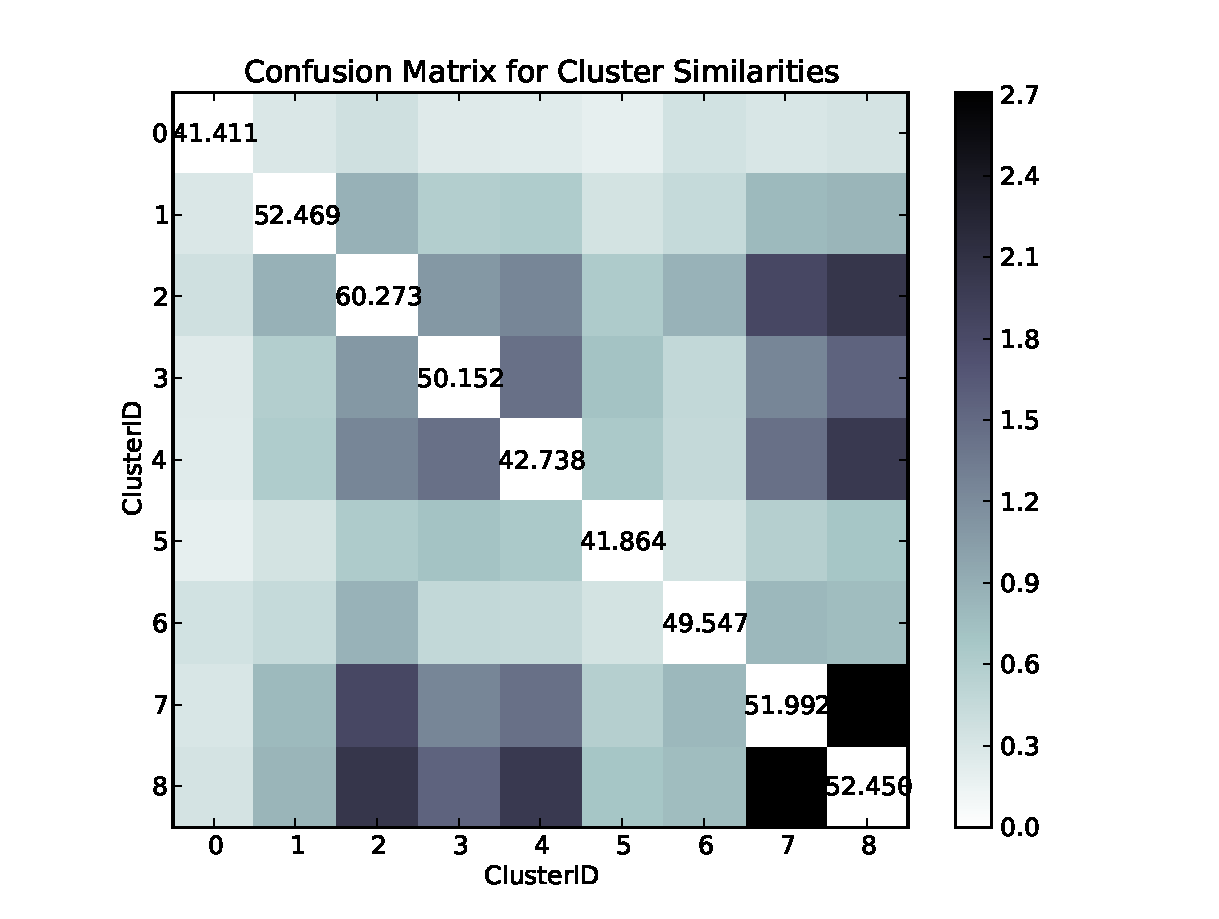
\includegraphics[width=0.48\linewidth]{clusts_nopca.pdf}}}
 \mbox{\subfigure[PCA]{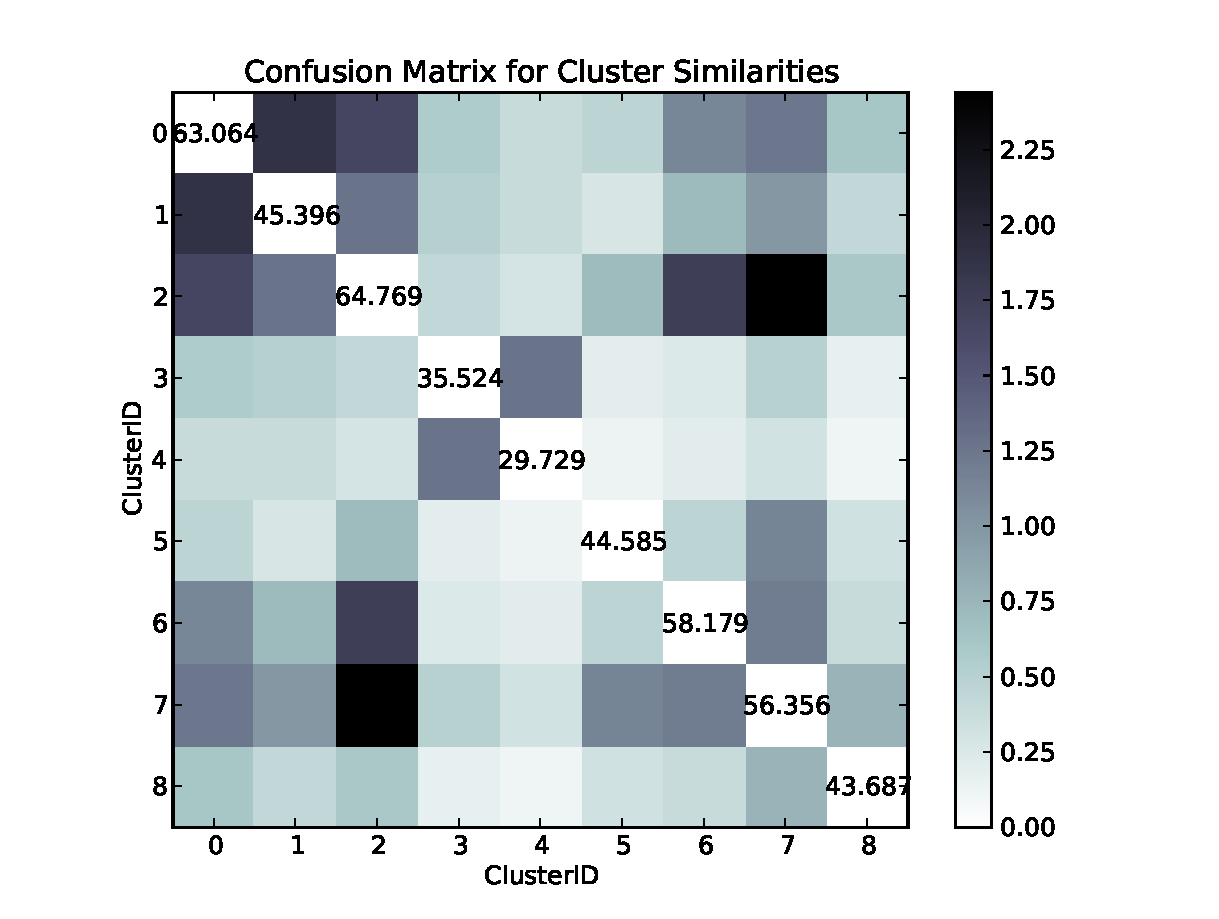
\includegraphics[width=0.48\linewidth]{clusts_pca.pdf}}}
 \caption{Matriz de confusão da similaridade entre grupos}
 \label{fig:conf}
\end{figure*}

Além disto, computamos também a correlação (usando o coeficiente de Pearson) entre o valor da entropia
de um grupo a sua similaridade média com os outros. Esta correlação foi de 0.58 e 0.87 para NONPCA e
PCA. Isto é um indicativa que o uso de PCA ajuda a minimizar a entropia de alguns grupos.

\subsection{Código}

\begin{verbatim}
src/dm/tp3/scripts/k_means.py
\end{verbatim}

\bibliographystyle{plain}
\bibliography{bibs}

\end{document}
